\pagebreak
\section{Utility analysis}

\subsection{Attribute utility table}
Under modifiability there were originally three attributes. The two attributes “Add Weapon” and “Add ingame objects” are both split into add simple and add advanced, weapons and ingame objects respectively. This is done following our meeting with A16. The attribute “Change GUI” is specific to simple changes to menu buttons and layout.

\begin{table}[H]
\small
\begin{tabular}{| p{0.18\textwidth} | p{0.3\textwidth} | p{0.12\textwidth} | p{0.4\textwidth} |} \hline
{\bf Attribute} & {\bf Scenario} & {\bf Priority} & {\bf Details} \\ \hline
Testability & Unit testing & (H,M) & 90\% bug discovery \\ \hline
Testability & Code coverage & (H,M) & 80\% of code covered by tests \\ \hline
Testability & Test game functionality & (H,L) & Tests should run in 30 seconds \\ \hline
Modifiability & Add simple weapon & (M,L) & Implemented and tested in 1 hour \\ \hline
Modifiability & Add advanced weapon & (L,H) & Implemented and tested in 5 hours \\ \hline
Modifiability & Add simple object & (M,L) & Implemented and tested in 1 hour \\ \hline
Modifiability & Add advanced object & (L,H) & Implemented and tested in 5 hours \\ \hline
Modifiability & Change GUI & (M,L) & Implement changes in 2 hours \\ \hline
\end{tabular}
\caption{Attribute utility table}
\end{table}

\normalsize

\pagebreak
\subsection{Attribute utility tree}

The utility tree corresponds to the table structure from the previous section.

\begin{figure}[H]
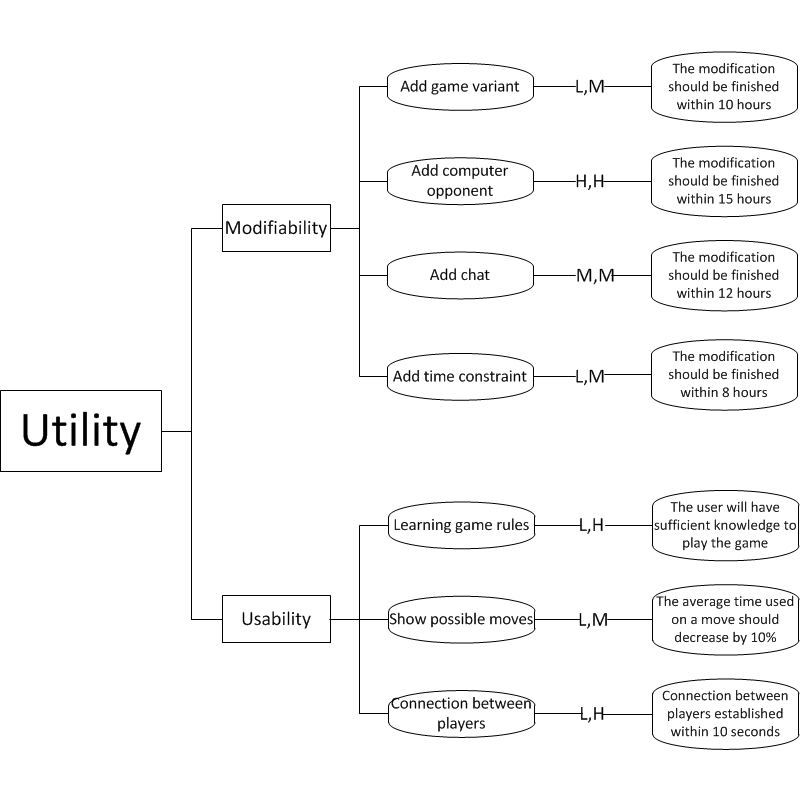
\includegraphics[width=1\textwidth]{Images/utility}
\caption{Attribute utility tree}
\end{figure}




